%%%%%%%%%%%%%%%%%%%%%%%%%%%%%%%%%%%%%%%%%
% Article EcoFoG
% Version 2.1 (23/10/2017)
%
% adapté de :
% Stylish Article
% LaTeX Template
% Version 1.0 (31/1/13)
%
% This template has been downloaded from:
% http://www.LaTeXTemplates.com
%
% Original author:
% Mathias Legrand (legrand.mathias@gmail.com)
%
% License:
% CC BY-NC-SA 3.0 (http://creativecommons.org/licenses/by-nc-sa/3.0/)
%
%%%%%%%%%%%%%%%%%%%%%%%%%%%%%%%%%%%%%%%%%


%----------------------------------------------------------------------------------------
%	PACKAGES AND OTHER DOCUMENT CONFIGURATIONS
%----------------------------------------------------------------------------------------

\documentclass[fleqn,10pt]{ArtEcoFoG} % Document font size and equations flushed left

\setcounter{tocdepth}{3} % Show only three levels in the table of contents section: sections, subsections and subsubsections


% Pandoc environments
\usepackage{framed}
\usepackage{fancyvrb}
\providecommand{\tightlist}{%
  \setlength{\itemsep}{0pt}\setlength{\parskip}{0pt}}
\newcommand{\VerbBar}{|}
\newcommand{\VERB}{\Verb[commandchars=\\\{\}]}
\DefineVerbatimEnvironment{Highlighting}{Verbatim}{commandchars=\\\{\}, fontsize=\scriptsize} % Code R
\definecolor{shadecolor}{RGB}{248,248,248}
\newenvironment{Shaded}{\begin{snugshade}}{\end{snugshade}}
\newcommand{\KeywordTok}[1]{\textcolor[rgb]{0.13,0.29,0.53}{\textbf{{#1}}}}
\newcommand{\DataTypeTok}[1]{\textcolor[rgb]{0.13,0.29,0.53}{{#1}}}
\newcommand{\DecValTok}[1]{\textcolor[rgb]{0.00,0.00,0.81}{{#1}}}
\newcommand{\BaseNTok}[1]{\textcolor[rgb]{0.00,0.00,0.81}{{#1}}}
\newcommand{\FloatTok}[1]{\textcolor[rgb]{0.00,0.00,0.81}{{#1}}}
\newcommand{\ConstantTok}[1]{\textcolor[rgb]{0.00,0.00,0.00}{{#1}}}
\newcommand{\CharTok}[1]{\textcolor[rgb]{0.31,0.60,0.02}{{#1}}}
\newcommand{\SpecialCharTok}[1]{\textcolor[rgb]{0.00,0.00,0.00}{{#1}}}
\newcommand{\StringTok}[1]{\textcolor[rgb]{0.31,0.60,0.02}{{#1}}}
\newcommand{\VerbatimStringTok}[1]{\textcolor[rgb]{0.31,0.60,0.02}{{#1}}}
\newcommand{\SpecialStringTok}[1]{\textcolor[rgb]{0.31,0.60,0.02}{{#1}}}
\newcommand{\ImportTok}[1]{{#1}}
\newcommand{\CommentTok}[1]{\textcolor[rgb]{0.56,0.35,0.01}{\textit{{#1}}}}
\newcommand{\DocumentationTok}[1]{\textcolor[rgb]{0.56,0.35,0.01}{\textbf{\textit{{#1}}}}}
\newcommand{\AnnotationTok}[1]{\textcolor[rgb]{0.56,0.35,0.01}{\textbf{\textit{{#1}}}}}
\newcommand{\CommentVarTok}[1]{\textcolor[rgb]{0.56,0.35,0.01}{\textbf{\textit{{#1}}}}}
\newcommand{\OtherTok}[1]{\textcolor[rgb]{0.56,0.35,0.01}{{#1}}}
\newcommand{\FunctionTok}[1]{\textcolor[rgb]{0.00,0.00,0.00}{{#1}}}
\newcommand{\VariableTok}[1]{\textcolor[rgb]{0.00,0.00,0.00}{{#1}}}
\newcommand{\ControlFlowTok}[1]{\textcolor[rgb]{0.13,0.29,0.53}{\textbf{{#1}}}}
\newcommand{\OperatorTok}[1]{\textcolor[rgb]{0.81,0.36,0.00}{\textbf{{#1}}}}
\newcommand{\BuiltInTok}[1]{{#1}}
\newcommand{\ExtensionTok}[1]{{#1}}
\newcommand{\PreprocessorTok}[1]{\textcolor[rgb]{0.56,0.35,0.01}{\textit{{#1}}}}
\newcommand{\AttributeTok}[1]{\textcolor[rgb]{0.77,0.63,0.00}{{#1}}}
\newcommand{\RegionMarkerTok}[1]{{#1}}
\newcommand{\InformationTok}[1]{\textcolor[rgb]{0.56,0.35,0.01}{\textbf{\textit{{#1}}}}}
\newcommand{\WarningTok}[1]{\textcolor[rgb]{0.56,0.35,0.01}{\textbf{\textit{{#1}}}}}
\newcommand{\AlertTok}[1]{\textcolor[rgb]{0.94,0.16,0.16}{{#1}}}
\newcommand{\ErrorTok}[1]{\textcolor[rgb]{0.64,0.00,0.00}{\textbf{{#1}}}}
\newcommand{\NormalTok}[1]{{#1}}
\usepackage{longtable,booktabs}
\usepackage{caption}
% These lines are needed to make table captions work with longtable:
\makeatletter
\def\fnum@table{\tablename~\thetable}
\makeatother
% longtable 2 columns
% https://tex.stackexchange.com/questions/161431/how-to-solve-longtable-is-not-in-1-column-mode-error
\makeatletter
\let\oldlt\longtable
\let\endoldlt\endlongtable
\def\longtable{\@ifnextchar[\longtable@i \longtable@ii}
\def\longtable@i[#1]{\begin{figure}[t]
\onecolumn
\begin{minipage}{0.5\textwidth}\scriptsize
\oldlt[#1]
}
\def\longtable@ii{\begin{figure}[t]
\onecolumn
\begin{minipage}{0.5\textwidth}\scriptsize
\oldlt
}
\def\endlongtable{\endoldlt
\end{minipage}
\twocolumn
\end{figure}}
\makeatother

\usepackage{graphicx,grffile}
\makeatletter
\def\maxwidth{\ifdim\Gin@nat@width>\linewidth\linewidth\else\Gin@nat@width\fi}
\def\maxheight{\ifdim\Gin@nat@height>\textheight0.8\textheight\else\Gin@nat@height\fi}
\makeatother
% Scale images if necessary, so that they will not overflow the page
% margins by default, and it is still possible to overwrite the defaults
% using explicit options in \includegraphics[width, height, ...]{}
\setkeys{Gin}{width=\maxwidth,height=\maxheight,keepaspectratio}

% User-adder preamble
\usepackage{textcomp} \DeclareUnicodeCharacter{B0}{\textdegree}
\hyphenation{sa-plings} \usepackage{longtable,tabu}

%----------------------------------------------------------------------------------------
%	ARTICLE INFORMATION
%----------------------------------------------------------------------------------------

\JournalInfo{\ }
\Archive{\ }

\PaperTitle{Inescapable Taxonomists: Workable Biodiversity Management Based on a
Minimum Field Work} % Article title

\Authors{
Ariane Mirabel\textsuperscript{1*}\\ Bruno Hérault\textsuperscript{2}\\ Eric Marcon\textsuperscript{1}
} % Authors
\affiliation{
\textsuperscript{1}UMR EcoFoG, AgroParistech, CNRS, Cirad, INRA, Université des Antilles,
Université de Guyane.\\ \hspace{1em} Campus Agronomique, 97310 Kourou, France.\\\textsuperscript{2}INPHB (Institut National Ploytechnique Félix Houphoüet Boigny)\\ \hspace{1em} Yamoussoukro, Ivory Coast
}
\affiliation{*\textbf{Corresponding author}: ariane.mirabel@ecofog.gf, https://github.com/ArianeMirabel} % Corresponding author

\Keywords{Biodiversity Measurement, Tree Community, Neotropical Forests, Botanical Uncertainty Propagation, Bayesian Estimator} % Keywords - if you don't want any simply remove all the text between the curly brackets
\newcommand{\keywordname}{Keywords} % Defines the keywords heading name

%----------------------------------------------------------------------------------------
%	ABSTRACT
%----------------------------------------------------------------------------------------

\Abstract{
Assess the fate of Neotropical forests requires to accurately measures
forest diversity and reliably monitor forest communities. The costs of
botanical inventories and the taxonomic complexity of Neotropical
forests make forest inventories in vernacular names the most efficient
approach today, although these hold high botanical uncertainty and limit
the accuracy of diversity measures. Several methods were proposed to
compensate these botanical uncertainties but none reliably assessed
functional and fine-scale diversity surveys. We developed a polyvalent
diversity estimator workable in numerous specific cases based on the
propagation of botanical uncertainties. The estimator was calibrated
with a large neotropical inventory and the simulations of uncertainty
and sampling effort gradients allowed to determined an ideal inventory
protocol optimizing the costs and the accuracy of forest inventories.
Our study first advocated of necessity of real inventories and the
inescapable recourse to taxonomists to ensure reliable diversity
estimations. An ideal inventory protocol based on a sampling effort of
XX trees and on an identification effort of 80\% of the species was
identified and ensured diversity estimations with a 10\% error.
}

%----------------------------------------------------------------------------------------

\begin{document}

\selectlanguage{english}

\flushbottom % Makes all text pages the same height

\maketitle % Print the title and abstract box

\tableofcontents % Print the contents section

\thispagestyle{empty} % Removes page numbering from the first page

%----------------------------------------------------------------------------------------
%	ARTICLE CONTENTS
%----------------------------------------------------------------------------------------


\section{Introduction}\label{introduction}

The variety of tree species, their assemblages in space and their
dynamics in time are determinant of forests productivity and functioning
\citep{Cardinale2012}. Preserve tree diversity is crucial to maintain
forests functioning and services, specifically in hyper-diverse tropical
forests where the biodiversity is as threatened as it is valuable and
unexplored \citep{Barlow2018}. Handling the conservation and management
of tree diversity requires setting sensible protection areas and
sustainable forest management calibrated according to diversity patterns
in space and time and their determinants
\citep{Margules2000, Purvis2000, Gibson2011a, FAO2014, Sist2015}.

Correctly measure, map and manage forests biodiversity require accurate
and large forest monitoring. The precision of forest inventories,
though, is often limited by their significant cost in terms of time,
money, and logistic \citep{Feeley2011, Baraloto2013}. Sampling methods
were optimized to minimize these costs and maximize inventory
accuracy.Some approaches would restrict inventories to some DBH or
height classes, to specific taxa, or would opt for inventories at family
or genus level. These methods efficiently translated biodiversity
patterns at regional scales and along wide ecological gradients
\citep{Steege2000, Higgins2004, Rejou-Mechain2011, Pos2014}. However,
these methods were either limited to small areas (under 1ha), sometimes
remained biased or holding significant uncertainty, and usually proved
limited to detect subtle diversity aspects and to desentangle richness
from equitability parameters
\citetext{\citealp{Phillips2003a}; \citealp{Baraloto2013}; \citealp[
]{Guitet2014b}; \citealp{Vellend2008}; \citealp{Prance1994}}. Another
approach proposed to use inventories in vernacular names instead of
botanical species. Vernacular names indeed are easier to attribute, more
common and usually do not require vouchers collection or posterior
botanical identification. The reliability of vernacular names may be
high at genus level, but this proved highly variable across tropical
regions: while this reliability was estimated around 60-70\% in French
Guiana \citep{Hawes2012, Guitet2014b} to ranges from 32\% to 67\% in
Central Africa \citep{Rejou-Mechain2011}. The multiple and variable
associations between botanical and vernacular names then entail
significant botanical uncertainties that should not be ignored
\citep{Oldeman1968}. Besides, rough vernacular inventories would not
allow functional and phylogenetic approaches, that require
identification at the botanical species to comply with phylogenetic and
functional database. However the approach through vernacular names
deserves further attention. First, it gives the opportunity to analyze
pre-logging inventories conducted in large areas by logging companies.
Second, as exhaustive inventories, they allow some post-process based on
vernacular/botanical names association and allow the building of
reliable diversity estimators
\citep{TerSteege2006, Feldpausch2006, Rejou-Mechain2008, Rejou-Mechain2011}.
Following this idea \citet{Guitet2014b} proposed a framework propagating
vernacular names taxonomic uncertainties in diversity measures. The
propagation framework was based on Monte-Carlo processes estimating
forest diversity from the vernacular-botanical name association. These
association combined prior information from both general taxa-abundance
correspondence table \citep{Molino2009} and reference field inventories.
The framework successfully rendered the ranking of plots diversity, but
remained restricted to large environmental gradient and for highly
different communities \citep{Guitet2014b, Guitet2013}. In this study we
offer to refine this framework and adapt it to diversity estimation at
smaller spatial scales. The following diversity estimator is based on
the specific case of the studied community and the inventory protocol.
The diversity estimator besides suits all inventories whatever the ratio
of botanical determination, \emph{i.e.} ratio of vernacular compared to
botanical names. It besides suits experimental specific as well as
pre-logging inventories where only the commercial or most recognizable
species are identified at species level.

Such diversity estimator allows maximizing the accuracy of diversity
measures while minimizing the sampling effort, \emph{i.e.} the size of
inventoried communities and the number of accurately identified species.
In this perspective we thought to calibrate an ideal inventory protocol
optimized in terms of sampling effort and determination degree. From a
real inventory, with complete vernacular and botanical identifications,
we simulated ranges of sampling efforts and identification degrees along
which we examined the bias and variability of the diversity estimator.

In this study we \emph{(i)} redesigned a diversity estimator based on a
Bayesian framework accounting for both general taxa-association tables
and specific field inventories, and \emph{(ii)} applied the estimator to
a real Neotropical forest inventory to determine the sampling effort and
determination degree of an ideal inventory protocol.

\section{Methods}\label{methods}

\subsection{Study community}\label{study-community}

We based our analyses on the inventory of a Neotropical rainforest, from
the Paracou Research Station in French Guiana (5°18'N and 52°53'W). The
experimental site stands in a lowland tropical rainforest with a flora
dominated by \emph{Fabaceae}, \emph{Chrysobalanaceae},
\emph{Lecythidaceae} and \emph{Sapotaceae} families. Mean mean annual
temperature is 26°C. and the mean annual precipitations average
\(2980 mm.y^-1\) (30-y period) with a 3-months dry season
(\(< 100 mm.months-1\)) from mid-August to mid-November and a one-month
dry season in March \citep{Wagner2011}. Elevation ranges between 5 and
50 m and soils correspond to thin acrisols over a layer of transformed
saprolite with low permeability, generating lateral drainage during
heavy rains \citep{IUSSWorkingGroupWRB2015}. We used the 2015 inventory
of six permanent plots of undisturbed forest (6.25ha each, 37.5ha
inventoried in total). During inventories trees are identified first
with a vernacular name assigned by the forest worker team, and afterward
with a scientific name assigned by botanists during regular botanical
campaigns. The community inventoried ancompasses 22 904 trees belonging
to 375 species and 63 families, identified by 290 different vernacular
names. The initial taxonomic uncertainty was 3\% of the community,
\emph{i.e.} the proportion of trees not identified with a botanical
name.

\subsection{Diversity measures}\label{diversity-measures}

Among the large panel of diversity indices we examined here the family
of q-generalized (Tsallis) entropy, widely adopted to assess all aspects
of taxonomic, functional and phylogenetic diversities. The Tsallis
diversity indices derive from a general formula, modulated by an order q
emphasizing species frequency \eqref{eq:TsallisEntropy}.

\begin{equation}
^qD = \sum_{i=1}^{N}{\left( p_i^q \right)^{\frac{1}{1-q}} }
\label{eq:TsallisEntropy}
\end{equation}

In the diversity formula, species relative abundance \(p_i\) in a
community of \(N\) species is raised at the power \(q\) that is the
order of the diversity. The higher the order \(q\), the higher the
emphasis on common vs.~rare species, so browsing a range of order \(q\)
corresponds assess a gradient balance between richness and evenness. The
formula retrieves species richness for \(q = 0\) , Shannon diversity for
\(q = 1\) where richness and evenness are equally accounted for and
Simpson diversity, that can be undestood as the diversity of common
species, for \(q = 2\). The Tsallis diversity indices would eventually
be converted into equivalent number of species in our framework. The
conversion in equivalent number of species, through Hill transformation,
allows understandable analysis and comparisons among communities
\citep{Hill1973, Keylock2005, Jost2006}.

\subsection{Diversity estimator}\label{diversity-estimator}

The estimation framework is based on the diversity distribution measured
on theoretical, fully determined communities. Theoretical inventories
are simulated 1 000 times from the real incomplete inventory, through
the replacement by a Monte-Carlo scheme of vernacular names by botanical
ones.

The vernacular-botanical replacement are based on the association
probability between each vernacular names and the botanical names
inventoried. For each vernacular name the association model follows a
multinomial distribution
\(M([s_1, s_2, …, s_N] ,[\alpha_1, \alpha_2,…, \alpha_N])\), with
\([\alpha_i]\) the association probability of botanical name \(s_i\)
with the vernacular name.

The association probability vectors \([\alpha_v]\) were determined with
a Bayesian framework based on the combination of botanical expertise and
observed associations. First, the estimation of \([\alpha_v]\) accounted
for prior information from experts' knowledge in the form of a general
taxa-association table listing all botanical names likely corresponding
to the vernacular name \(v\). From this general table, the probability
\(\lambda_i={}^1/m_v\) was attributed to each of the \(m_v\) botanical
names with a confirmed association with \(v\). When no association was
established the probability \(\lambda_i={}^\epsilon\big/_{N-m_v}\) was
attributed to the botanical name, with \(\epsilon\) standing for a
background noise set to 0.01 here. Second, the estimation of
\([\alpha_v]\) accounted for observed inventories giving real
association frequencies \(\phi_i\) between \(v\) and the \(m_v'\)
botanical names with observed association. Similarly, the association
probability \(\lambda_i={}^\epsilon\big/_{N-m_v'}\) was attributed to
botanical names with no observed association. The final \([\alpha_v]\)
distribution was modeled by a Multinomial-Dirichlet scheme combining the
two vectors \([\lambda^v]\) and \([\phi^v]\) \citep{McCarthy2007}.

To test the relevance of the general table and observed inventories
information, we tested a range of weighting \(w\). Assuming a
distribution of \([\phi^v]\) conditionally to \([\alpha^v]\) the
weighting returned the formula \eqref{eq:weighting}.

\begin{equation}
[\alpha_i^v]: 
\Big[\alpha_i^v | _{(1-w)\lambda_i^v ,w.\phi_i^v}\Big] =Dirichlet\Big((1-w)\phi_i^v+w.\lambda_i^v\Big)
\label{eq:weighting}
\end{equation}

When \(w=0\) only observed inventories were considered, when \(w=0.5\)
both information were equally accounted for and when \(w=1\) only the
general taxa-association table was considered.

\subsection{Simulation of determination and sampling effort
gradients}\label{simulation-of-determination-and-sampling-effort-gradients}

The estimator was calibrated in comparing several methods for the
vernacular/botanical association probability (corresponding to different
values of \(w\), the balance between general table and observed
inventories). The performance of the estimator was examined regarding
its bias, \emph{i.e.} the difference between the estimation and the real
diversity, and its variability, \emph{i.e.} 95\% confidence interval
\citep{Baltanas2009}. For each computation method the performance of the
estimator was examined along a determination gradient (corresponding to
an increasing number of species only identified in vernacular name). As
rare species had more chance to be undetermined (Kendall test,
\(\tau = -0.46, p < 10^-16\)), the trial of ignored determination
followed botanical names abundance (\(p_{undetermined}=f_i^{-0.1}\),
with \(f_i\) botanical name frequency).

Different inventory specific cases were then tested in examining the
bias and variability of the estimator along a sampling effort gradient
(corresponding to an increasing number of trees, from 500 to 22 000
trees, used to compute the vernacular/botanical association
probability). Along the sampling effort gradient the estimations were
performed on the fully undetermined inventory, \emph{i.e.} without any
botanical identification.

\section{Results}\label{results}

\subsection{The reponse to determination effort, and the design of an
ideal
framework}\label{the-reponse-to-determination-effort-and-the-design-of-an-ideal-framework}

Along the indetermination gradient, when considering both general
taxa-association table and observed inventory the diversity was
increasingly overestimated (Fig. \ref{fig:UncertGrad}). This
overestimation increased with the order of diversity q, while it was not
significant for the richness (\(q=0\)), the overestimation reached 45\%
of the real diversity for Shannon diversity (\(q = 1\)) and it reached
57\% of the real diversity for the Simpson diversity (\(q = 2\)).

When only considering the general taxa-association table the richness
(\(q=0\)) was underestimated (reaching a 50\% underestimation), while
both Shannon and Simpson diversities were overestimated (respectively
reaching underestimations of 67\% and 125\%).

When only considering the observed inventory the estimator remained
slightly biased but it did not exceed 15\% of the real diversity for any
order of diversity.

A bootstrap of the 100 simulations for each specific case and diversity
order showed a stabilization of variances after 60 simulations.

\begin{figure*}
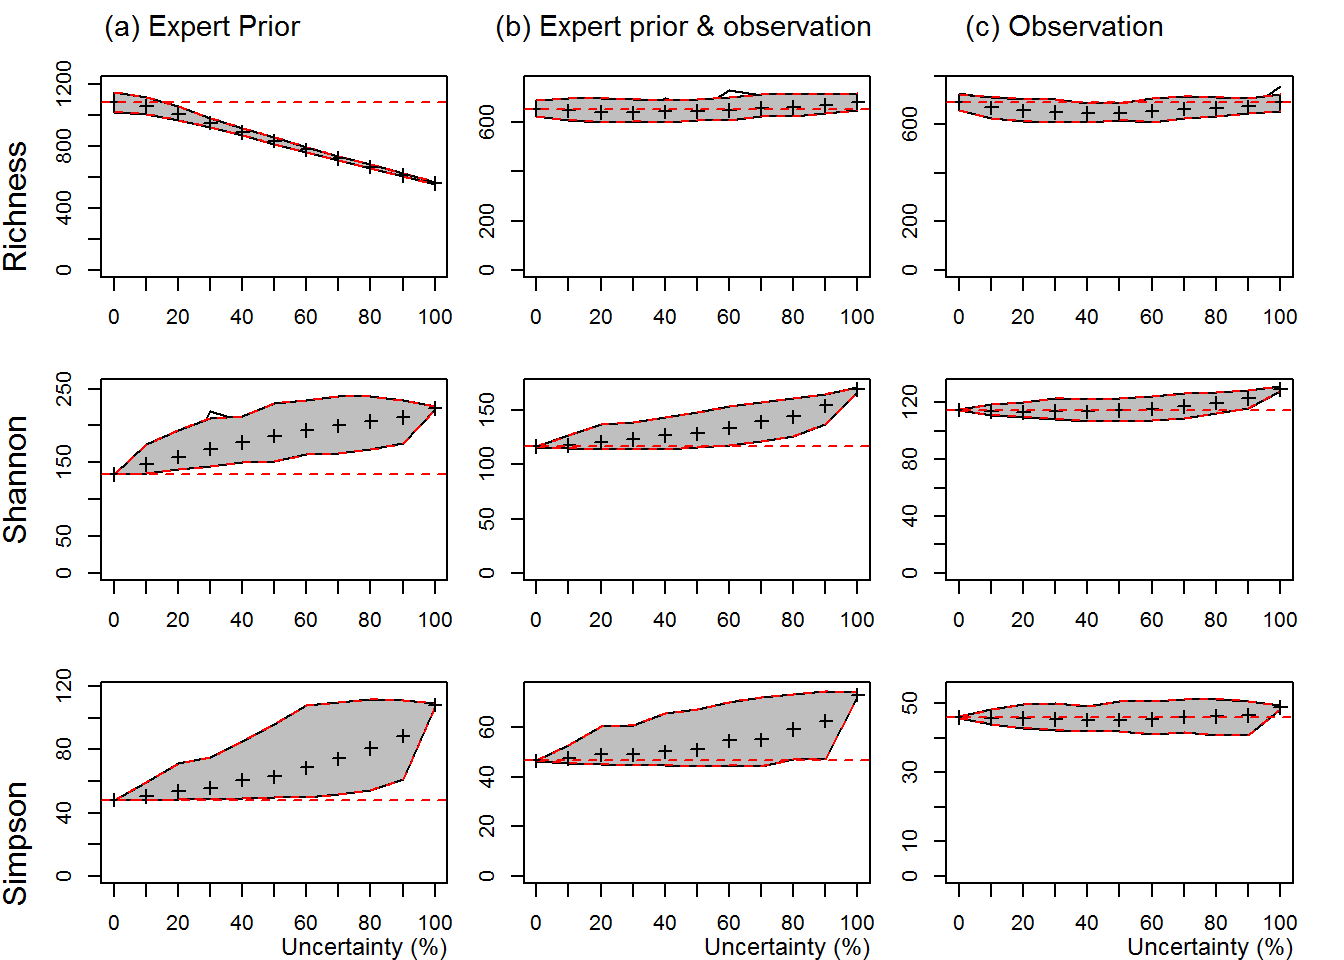
\includegraphics[width=1\linewidth]{TaxonomicUncertainty_files/figure-latex/UncertGrad-1} \caption{Richness, Shannon and Simpson estimator bias and 95\%confidence interval along an uncertainty gradient with the association frequencies computed from (a) only expert prior, (b) both expert and observation prior and (c) only observation prior.}\label{fig:UncertGrad}
\end{figure*}

\subsection{Calibrating the sampling
effort}\label{calibrating-the-sampling-effort}

Along the sampling effort gradient from 500 to 22 000 trees, the
richness estimator remained negatively biased but the confidence
interval did not exceed 7\%. The Shannon and Simpson were less biased,
for 3 000 trees inventoried the Shannon diversity bias fell to 15\%
while the bias of Simpson estimator fell to 6\% (Fig.
\ref{fig:SEgradient}).

\begin{figure*}
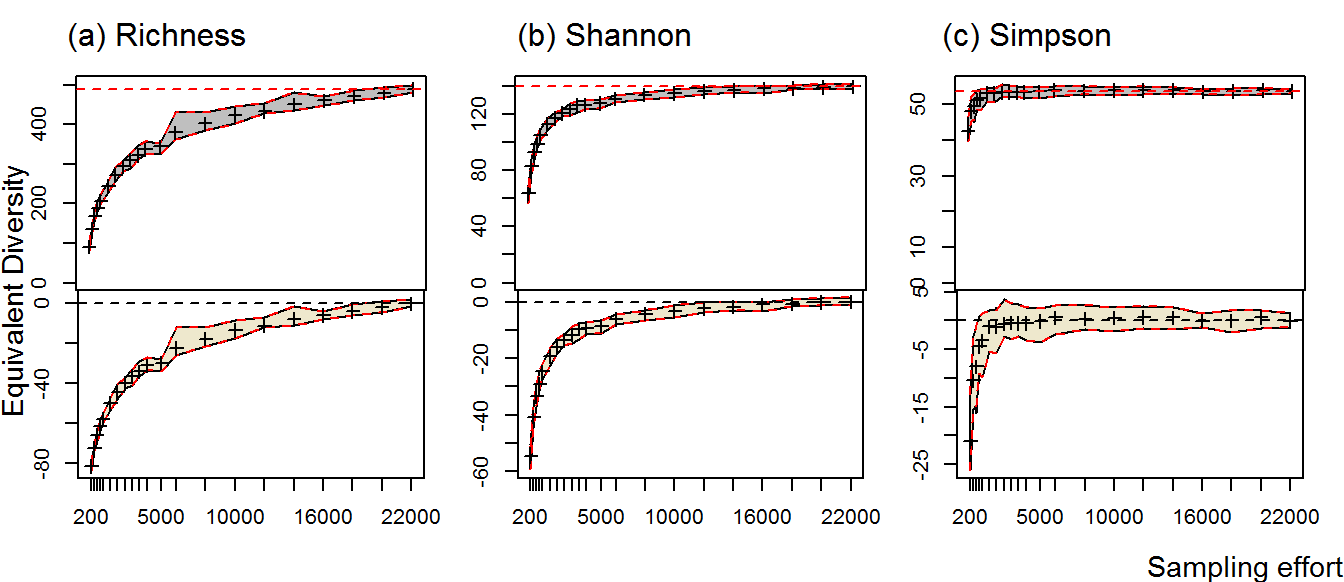
\includegraphics[width=1\linewidth]{TaxonomicUncertainty_files/figure-latex/SEgradient-1} \caption{Richness, Shannon and Simpson estimation (upper panels) and bias compared to real diversity (lower panels) along a sampling effort gradient. Shaded areas are the 95\% confidence intervals, vertical plain line stands for the points at 3 000 trees.}\label{fig:SEgradient}
\end{figure*}

The precision and bias of the estimator were eventually tested for the
recomended sampling effort of 3 000 trees. In this case the Shannon and
Simpson biases remained lower than 10\% and the Richness bias was below
10\% until 20\% of undetermined species.

\begin{figure}
\centering
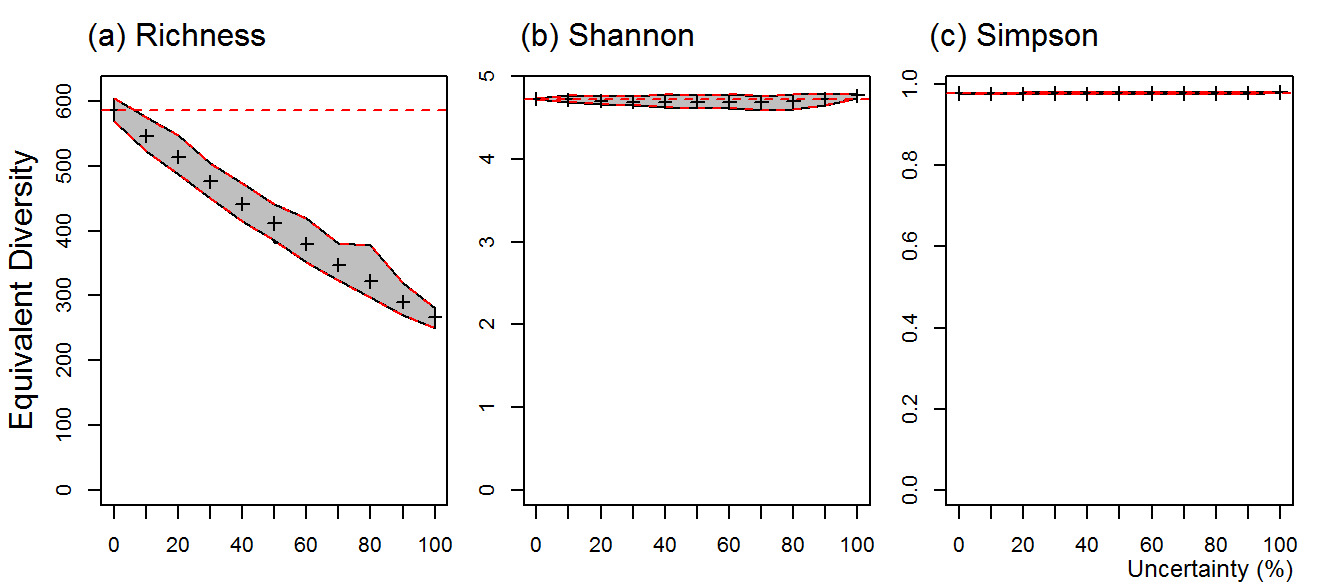
\includegraphics{TaxonomicUncertainty_files/figure-latex/UncertGradLim-1.pdf}
\caption{\label{fig:UncertGradLim}Richness, Shannon and Simpson estimators
along a taxonomic uncertainty gradient based on field inventories of 3
000 trees, with shaded areas the 95\% confidence interval.}
\end{figure}

\section{Discussion}\label{discussion}

\subsection{Inescapable taxonomists}\label{inescapable-taxonomists}

The method developed in the line of \citet{Guitet2014b} to propagate the
taxonomic uncertainty of vernacular names in diversity mesures provided
a reliable estimator for diversity indices, workable for all diversity
order and adaptable for functoinal diversity. The use the general
taxonomic-association table proved to systematically overestimate the
diversity. In these tables the vernacular/botanical association
probabilities were independent of botanical name abundances, so rare
vernacular names were indifferently replaced by rare or abundant
botanical names. As a result, the abundance of rare species were
inflated at the expense abundant ones, which overestimated the
equitability. Contrastingly the use of observed inventories that account
for the abundance of botanical names proved more reliable. The rescourse
to taxonomists and pre-inventories proved unavoidable to correctly
estimate and therefore manage forest biodiversity.

\subsection{Calibration of an optimized inventory
protocol}\label{calibration-of-an-optimized-inventory-protocol}

The performance of the estimator, regarding its bias and variability,
along the determination and sampling efforts gradients highlighted the
difficulty to assess communities richness. Whatever the inventory
protocol the richness indeed remained significantly biased, as already
suggested in previous analysis comparing several inventory methods
\citep{Higgins2004}.

Conversely, the Shannon and Simpson diversity estimations proved less
biased, thus allowing the estimator to detect small variation of
community equitability. This would be a key to value existing
inventories and ease future protocols as subtle time and spatial
diversity variations often invlove changes in community abundance
distribution rather than richness
\citep{Baraloto2012a, Berry2008a, Cannon1998, Plumptre1996}.

An optimized protocol maximizing the estimator performance on the one
hand and minimizing the determination and sampling efforts on the other
hand corresponding to the pre-inventory of at least 3 000 trees and the
determination of 80\% of the botanical species.

\section{Conclusion}\label{conclusion}

The diversity estimator developed in this paper (i) proved relevant to
measure tropical forest diversity at small time and spatial scale, (ii)
allowed to integrate the specificities of local forests and working
team, and (iii) was adaptable for both taxonomic and functional
diversity at all order. Examining the estimator performance highlighted
the inescapable rescourse to taxonomists and to minimum real
inventories: an initial inventory of 3 000 trees with 80\% of the
species identified allowed an estimation accurate at 10\% of Shannon and
Simpson diversities. The diversity estimator allows integrating and is
thus adaptable to all specific case.

%----------------------------------------------------------------------------------------
%	REFERENCE LIST
%----------------------------------------------------------------------------------------

\bibliographystyle{mee}
\makeatletter
% The filename has .bib extension the must be eliminated
\filename@parse{references.bib}
% parse stores the file name in base. Extension starts at the first dot, so don't use dots in file names.
\bibliography{\filename@base}
\makeatother


%----------------------------------------------------------------------------------------

\end{document}
